
\section{SEO and Accessibility}
\subsection{SEO}
Apart from using Server-Side Rendering (SSR), we also use dynamic titles, meta keywords, and a sitemap to boost SEO.
\begin{figure}[h]
	\centering
	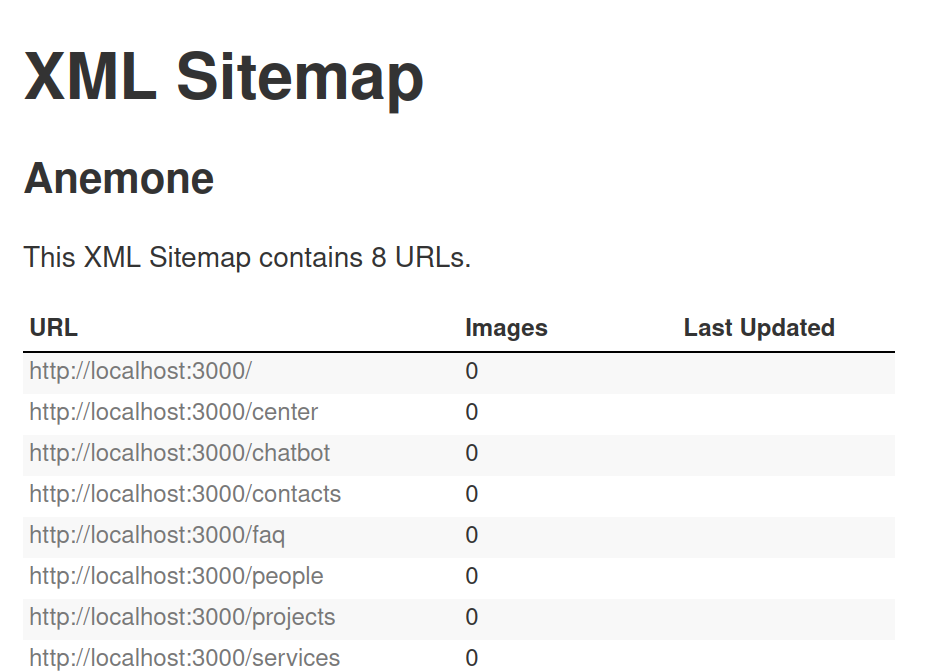
\includegraphics[width=\linewidth]{Resources/sitemap.png}
	\caption{The sitemap of our website.}
	\label{fig:example}
\end{figure}
\subsection{Accessibility}
We did some work on accessibility:

\begin{enumerate}
	\item Provide Alternative Text: Ensure all images have descriptive alt text so screen readers can convey the information to visually impaired users.
	\item Use Semantic HTML: Use semantic HTML tags like header, nav, main, article, and section to help screen readers understand the structure of the page.
	\item Add ARIA (Accessible Rich Internet Applications) Tags
\end{enumerate}





